\documentclass[12pt]{article}
\usepackage{amsmath,amssymb}
\usepackage{color}
\usepackage{tikz}
\usetikzlibrary{positioning}

\newcommand{\andy}[1] {\textcolor{red}{ #1 }} 

\begin{document}

\title{\textbf{Notes on the MARL Book\footnote{
Multi-Agent Reinforcement Learning: Foundations and Modern Approaches. 
Authors: Stefano V. Albrecht,  Filippos Christianos,  Lukas Schäfer. 
Published by MIT Press, 2024}
}} 
\author{Zeyu Liang}
\date{Monday, November 25, 2024}

\maketitle

%the 1st figure
\section*{Bellman Equation}
\[
v^\pi = r^0 + \gamma r^1 + \gamma^2 r^2 + \cdots = r^0 + \gamma v^{\pi, 1}
\]

Given a policy $\pi$, the state-value function $V^\pi(s)$ gives the ``value'' of the state $s$ under policy $\pi$:
\[
V^\pi(s) = \mathbb{E}_\pi\left[G_t \mid S_t = s\right] = \mathbb{E}_\pi\left[r_t + \gamma r_{t+1} + \gamma^2 r_{t+2} + \cdots \mid S_t = s\right]
\]
\[
= \sum_{a \in \mathcal{A}} \pi(a \mid s) \sum_{s' \in \mathcal{S}} T(s' \mid s, a) \left[ R(s, a, s') + \gamma \mathbb{E}_\pi\left[G_{t+1} \mid S_{t+1} = s'\right] \right]
\]
\[
= \sum_{a \in \mathcal{A}} \pi(a \mid s) \sum_{s' \in \mathcal{S}} T(s' \mid s, a) \left[ R(s, a, s') + \gamma V^\pi(s') \right]
\]
\textit{This is called Bellman Equation.}

\bigskip

\noindent
\textbf{Why is Bellman Equation useful?} \\
Because we can use a system of linear equations to solve for $V^\pi(\mathcal{S})$:
\[
\begin{cases} 
V^\pi(s_1) = \sum_{a \in \mathcal{A}} \pi(a \mid s_1) \sum_{s' \in \mathcal{S}} T(s' \mid s_1, a) \left[ R(s_1, a, s') + \gamma V^\pi(s') \right] \\
\vdots \\
V^\pi(s_k) = \sum_{a \in \mathcal{A}} \pi(a \mid s_k) \sum_{s' \in \mathcal{S}} T(s' \mid s_k, a) \left[ R(s_k, a, s') + \gamma V^\pi(s') \right] 
\end{cases}
\]

\bigskip

\noindent
Similarly, we can define \textit{action-value functions}:
\[
Q^\pi(s, a) = \mathbb{E}_\pi\left[ R(s, a, s') + \gamma \mathbb{E}_\pi\left[ G_{t+1} \mid S_{t+1} = s' \right] \mid S_t = s, A_t = a \right]
\]
\[
= \sum_{s' \in \mathcal{S}} T(s' \mid s, a) \left[ R(s, a, s') + \gamma V^\pi(s') \right]
\]

\bigskip

\noindent
\textbf{Iterative policy evaluation}: Repeatedly updates sweep \textit{all states} $s$:
\[
V^{k+1}(s) \leftarrow \sum_{a \in \mathcal{A}} \pi(a \mid s) \sum_{s' \in \mathcal{S}} T(s' \mid s, a) \left[ R(s, a, s') + \gamma V^k(s') \right]
\]
\textit{Round function, discount factor}

\bigskip

\noindent
\textbf{TD algorithms}: Temporal Difference, does not rely on knowing all MDP (reward functions, transition probability, etc)

\noindent
\textbf{action value function updates}:
\[
Q(S_t, A_t) \leftarrow Q(S_t, A_t) + \alpha \left( \mathcal{X} - Q(S_t, A_t) \right)
\]
where $\mathcal{X} = r_t + \gamma Q(S_{t+1}, A_{t+1})$

\bigskip

\noindent
\textbf{Algorithm Sarsa for MDPs (with $\varepsilon$-greedy policies)}
\begin{enumerate}
    \item Initialize $Q(S, a) = 0$ for all $s \in \mathcal{S}$ and $a \in \mathcal{A}$
    \item Repeat for every episode:
    \item Observe initial state $S^0$
    \item With probability $\varepsilon$: choose random action $a^0 \in \mathcal{A}$
    \item Otherwise: choose $a^0 \in \arg\max_a Q(S^0, a)$
    \item For $t = 0, 1, 2, \ldots$ do:
    \item Apply $a^t$, observe reward $r^t$ and next state $S^{t+1}$
    \item With probability $\varepsilon$: choose random action $a^{t+1} \in \mathcal{A}$
    \item Otherwise: choose $a^{t+1} \in \arg\max_a Q(S^{t+1}, a)$
    \item $Q(S^t, a^t) \leftarrow Q(S^t, a^t) + \alpha \left( r^t + \gamma Q(S^{t+1}, a^{t+1}) - Q(S^t, a^t) \right)$
\end{enumerate}

\bigskip

\noindent
\textbf{Understanding}: With $\varepsilon$ probability \textit{explore new action}, otherwise choose the \textit{current best} action.

%the 2nd figure
\section*{2.6 Difference between Q-learning and Sarsa}
On page 35 bottom.

\textbf{Algorithm DP Value Iteration for MDPs}
\begin{enumerate}
    \item Initialize \( V(s) = 0 \) for all \( s \in \mathcal{S} \).
    \item Repeat until \( V \) converged: \\
    \( \forall s \in \mathcal{S}: V(s) \leftarrow \max_{a \in \mathcal{A}} \sum_{s' \in \mathcal{S}} T(s'|s,a) \left[ R(s,a,s') + \gamma V(s') \right] \)
    \item Return optimal policy \( \pi^* \) with \\
    \( \forall s \in \mathcal{S}: \pi^*(s) \leftarrow \arg\max_{a \in \mathcal{A}} \sum_{s' \in \mathcal{S}} T(s'|s,a) \left[ R(s,a,s') + \gamma V(s') \right] \)
\end{enumerate}

In POSG, let \( \hat{h}^t = \{ s^0, a^0, s^1, a^1, \dots, s^t, a^t \} \) denote a full history up to time \( t \). \( O(\hat{h}^{t+1}) \) returns the history of joint observations. \\

Define the probability of joint observation: \( O(o^t | \hat{h}^t, s^t) = \prod_{i \in \mathcal{I}} O_i(o^t_i | o^{t-1}, s^t) \)

\textbf{Define History-based expected return for agent \( i \) as:} \\
\( V_i(\pi) = \sum_{\hat{h}^t \in \mathcal{H}} \Pr(\hat{h}^t | \pi) M_i(\hat{h}^t) \) \\
where \( \Pr(\hat{h}^t | \pi) \) is the probability of full history \( \hat{h}^t \) under \( \pi \). \\

\[ \Pr(\hat{h}^t | \pi) = \mu(s^0) O(o^0 | a^0, s^0) \prod_{\tau = 1}^t \pi(a^\tau | h^\tau) T(s^{\tau + 1} | s^\tau, a^\tau) O(o^\tau | o^{\tau - 1}, s^{\tau + 1}) \] \\

and \( M_i(\hat{h}^t) \) is the discounted return for agent \( i \) in \( \hat{h}^t \): \\
\[ M_i(\hat{h}^t) = \sum_{\tau = 0}^t \gamma^\tau R^i(s^\tau, a^\tau, s^{\tau + 1}) \] \\

\( \pi(a^t | h^t) \) is the probability of joint action \( a^t \) under \( \pi \) after joint observation \( h^t \)

%the 3rd figure
\bigskip
\section*{Recursive Expected Return}

\begin{itemize}
    \item Define \( \text{BR}_i(\pi_{-i}) = \arg\max_{\pi_i} U_i(\pi_i, \pi_{-i}) \quad \text{BR : Best Response} \)

    \item In a zero-sum two agents game, a joint policy \( \pi = (\pi_i, \pi_j) \) is a minimax solution, \\
    if \( U_i(\pi) = \max_{\pi_i} \min_{\pi_j} U_i(\pi_i, \pi_j) = \min_{\pi_j} \max_{\pi_i} U_i(\pi_i, \pi_j) = -U_j(\pi) \)

    \item \textbf{Minimax via Linear Programming} \\
    \( \min U_j^* \) \\
    subject to \( \sum_{a_i \in A_i} R_j(a_i, a_j) \pi_i(a_i) \leq U_j^* \quad \forall a_j \in A_j \) \\
    \( \chi_{a_j} \geq 0, \sum_{a \in A_i} \chi_a = 1 \)

    \item \textbf{Define: Nash Equilibrium} In a general sum game with \( n \) agents, a joint policy \( \pi = (\pi_1, \cdots, \pi_n) \) is a Nash Equilibrium if \\
    \( \forall i, \pi_i': U_i(\pi_i', \pi_{-i}) \leq U_i(\pi) \)

    \item \( \boldsymbol{\varepsilon}\)-\textbf{Nash Equilibrium}: \( \forall i, \pi_i': U_i(\pi_i', \pi_{-i}) - \varepsilon \leq U_i(\pi) \)

    \item \textbf{Correlated Equilibrium}: In a general sum game with \( n \)-agents, let \( \pi_C(a) \) be a joint policy that assigns probabilities to joint actions \( a \in A \). Then, \( \pi_C \) is a correlated equilibrium if for every agent \( i \in \mathcal{I} \) and every action modifier \( \xi_i: A_i \to A_i \) \\
    \( \sum_{a \in A} \pi_C(a) R_i(\xi_i(a_i), a_{-i}) \leq \sum_{a \in A} \pi_C(a) R_i(a) \) \\
    Correlated Equilibrium allows correlation between policies whereas Nash-Equilibrium doesn't.

    \item \textbf{Linear Programming for Correlated Equilibrium} \\
    maximize \( \sum_{a \in A} \sum_{i \in \mathcal{I}} \chi_a R_i(a) \quad \chi_a = \pi(a) \text{ representing selecting action } a \text{ under policy } \pi \) \\
    subject to \( \sum_{a \in A} \chi_a R_i(a) \geq \sum_{a \in A} \chi_a R_i(a_i', a_{-i}) \quad \andy{??} \)

    \item \textbf{Pareto Optimality}: A joint policy \( \pi \) is Pareto dominated by another policy \( \pi' \) \\
    if \( \forall i: U_i(\pi') \geq U_i(\pi) \) and \( \exists i: U_i(\pi') > U_i(\pi) \) \\
    \( \pi' \) is better than \( \pi \) because everyone gets more. \\
    \( \pi \) is Pareto optimal if it's not Pareto-dominated by any other policy

    \item Welfare of \( \pi \): \( W(\pi) = \sum_{i \in \mathcal{I}} U_i(\pi) \)

    \item Fairness of \( \pi \): \( F(\pi) = \prod_{i \in \mathcal{I}} U_i(\pi) \) \\
    If Welfare is fixed, fairness is maximum if all \( U_i(\pi) \) are equal. \\
    Welfare Optimality \( \implies \) Pareto Optimality, but not vice versa.

    \item Regret: \( = \max_{a_i \in A_i} \sum_{t=1}^2 \left[ R_i(a_i, a_{-i}^e) - R_i(a^e) \right] \) \\
    \text{if knows future, choose again.} \qquad \qquad \text{history} \\
    No Regret if \( \forall i: \lim_{z \to \infty} \frac{1}{z} \text{Regret}_i^z \leq 0 \). Refer Fig 4.6. 
\end{itemize}

%4th fig.
\bigskip
\section*{Central Learning, CQ-Learning}
\begin{enumerate}
    \item Initialize \( Q(S, a) = 0 \) for all \( s \in \mathcal{S} \) and \( a \in \mathcal{A}=A_1\times\cdots\times A_n \).
    \item Repeat for every episode.
    \item For \( t = 1,\cdots \) do
    \item Observe current state \( s^t \).
    \item With probability \( \varepsilon \): choose random action \( a^t \in \mathcal{A} \)
    \item Otherwise, choose \( a^t \in \arg\max_a Q(s^t, a) \)
    \item Apply joint action \( a^t \), observe rewards \( r^t_1,\cdots,r^t_n \) and \( s^{t + 1} \)
    \item Transform \( r^t_1\cdots r^t_n \) to \( r \) \textit{This step is usually unclear for general-sum game.}
    \item \( Q(s^t, a^t)\leftarrow Q(s^t, a^t)+\alpha\left[r^t+\gamma\max_{a'}Q(s^{t + 1}, a')-Q(s^t, a^t)\right] \)
\end{enumerate}

\noindent
Another limitation is that action space grows exponentially. \\
Also, Central policy to agents communication might not be feasible.

\bigskip

\noindent
\textbf{Independent Learning, IQL} \\
The algorithm is essentially the same with Q-learning. Algorithm control agent \( i \).

\bigskip

\noindent
\textbf{6.1 Value iteration for stochastic games}
\begin{enumerate}
    \item Initialize \( V_i(s)=0 \) for all \( s \in \mathcal{S} \) and \( i \in \mathcal{I} \)
    \item Repeat until all \( V_i \) have converged
    \item For all \( s \in \mathcal{S}, i \in \mathcal{I} \), joint action \( a \in \mathcal{A} \) do \\
    \( M_{s,i}(a)\leftarrow\sum_{s'\in \mathcal{S}}T(s'|s,a)\left[R_i(s,a,s')+\gamma V_i(s')\right] \)
    \item For all \( s \in \mathcal{S} \) and \( i \in \mathcal{I} \) \\
    \( V_i(s)\leftarrow\text{Value}(M_{s,1},\cdots,M_{s,n}) \)  % 原文“Value”未明确具体操作,保留英文
\end{enumerate}

\noindent
\( M_{s,i}(a) \) is the entry for matrix contains states and agents for rows and columns. \\
\( M_{s,i}(a) \) represents an approximation of return for agent \( i \) choosing joint action \( a \) after state \( s \).

%5th fig.
\bigskip

\section*{Joint-action learning}
It is a family of MARL algorithms based on temporal-difference learning. 
follows from Bellman Equation, the expected return for agent \( i \) when selecting 
joint action \( a=(a_1,\cdots,a_n) \) in state \( s \) and subsequently follow joint policy \( \pi \) is \\
\[ Q_i^\pi(s,a)=\sum_{s'\in S}T(s'|s,a)\left[R_i(s,a,s')+\gamma\sum_{a''\in A}\pi(a''|s')Q_i^\pi(s',a'')\right] \]


\textbf{The underlying idea in JAL-GT (joint action learning game theory)} is that the set of joint-action \\
joint-action values \( Q_1(s,\cdot),\cdots,Q_n(s,\cdot) \) can be treated as a non-repeated normal-form game. \\
\( \Gamma_s \) for state \( s \), in which the reward function for agent \( i \) is given by \\
\( R_i(a_1,\cdots,a_n)=Q_i(s,a_1,\cdots,a_n) \), (sometime noted as \( \Gamma_{s,i}(\cdot) \))

\bigskip
\textbf{Algorithm JAL-GT (controls agent \( i \))}
\begin{enumerate}
    \item Initialize \( Q_j(s,a) = 0 \) for all \( s\in S \), \( a\in A \)
    \item Repeat for every episode:
    \item for \( t = 0,1,2\cdots \) do:
    \item observe current state \( s^t \)
    \item With prob \( \varepsilon \): choose random action \( a_i^t \)
    \item Otherwise: solve \( \Gamma_{s^t} \) to get policies \( (\pi_1,\cdots,\pi_n) \), then sample action \( a_i^t\sim\pi_i \)
    \item Observe joint action \( a^t=(a_1^t,\cdots,a_n^t) \), rewards \( r_1^t,\cdots,r_n^t \), next state \( s^{t + 1} \)
    \item for all \( j\in\mathcal{I} \) do
    \item \( Q_j(s^t,a^t)\leftarrow Q_j(s^t,a^t)+\alpha\left[r_j^t+\gamma Q_j(s^{t + 1},a^{t + 1})-Q_j(s^t,a^t)\right] \)
\end{enumerate}

For example, a two agent \( i \) and \( j \) and three possible actions for each agent. \( \Gamma_s = [\Gamma_{s,i},\Gamma_{s,j}] \)

\[
\Gamma_{s,i}=\begin{bmatrix}
Q_i(s,a_{i,1},a_{j,1}), & Q_i(s,a_{i,1},a_{j,2}), & Q_i(s,a_{i,1},a_{j,3}) \\
Q_i(s,a_{i,2},a_{j,1}), & Q_i(s,a_{i,2},a_{j,2}), & Q_i(s,a_{i,2},a_{j,3}) \\
Q_i(s,a_{i,3},a_{j,1}), & Q_i(s,a_{i,3},a_{j,2}), & Q_i(s,a_{i,3},a_{j,3})
\end{bmatrix}
\]


\textbf{Difference between Minmax-Q-learning and Q-learning (Littman 1994)} \\
Minmax-Q is robust to optimal opponent, but can not analysis opponent weakness. 
Q-learning vice versa.


\textbf{Agent modeling}, based on history, belief, goal. \\
\textbf{Policy reconstruction of \( j \)}: learning parameters of \( \hat{\pi}_j \) can be framed 
as a supervised learning based on \( (s_j^t,a_j^t) \) data, history of state and action \\

Let \( C(s,a_j) \) denote the number of times that agent \( j \) selected action \( a_j \) in state \( s \). 
Then, the agent \( \hat{\pi}_j \) is defined as \( \hat{\pi}_j(a_j|s)=\frac{C(s,a_j)}{\sum_{a_j'\in A_j}C(s,a_j')} \) \\
See Fig 6.6 for example. 

%6th fig.
\bigskip
\section*{Algorithm JAL-AM (controls agent \( i \))}
\begin{enumerate}
    \item Initialize:
    \item \( Q_j(s,a) = 0 \) for all \( s \in \mathcal{S}, a \in \mathcal{A} \)
    \item Agent set \( \hat{\pi}_j(a_j|s) = \frac{1}{|\mathcal{A}_j|} \) for all \( j \neq i \) and \( s \in \mathcal{S} \).
    \item Repeat for every episode:
    \item For \( t = 0,1,2,\cdots \) do:
        \item Observe current state \( s^t \).
        \item \( \varepsilon \)-greedy explore
        \item Otherwise, choose \( \text{BR } a_i^t \in \arg\max_{a_i} AV_i(s^t,a_i) \)
        \item Observe joint action \( a^t=(a_1^t,\ldots,a_n^t) \), \( r_i^t \) and \( s^{t + 1} \)
        \item For \( j \neq i \) do:
            \item update \( \hat{\pi}_j \) agent model
            \item \( Q_j(s^t,a^t) \leftarrow Q_j(s^t,a^t) + \alpha \big[ r_i^t + \gamma \max_{a_i'} AV_i(s^{t+1},a_i') - Q_i(s^t,a^t) \big] \)
\end{enumerate}

where \( AV_i(s,a_i) = \sum_{a_{-i} \in \mathcal{A}_{-i}} Q_i(s,(a_i,a_{-i})) \prod_{j \neq i} \hat{\pi}_j(a_j|s) \)

- After observing agent \( j \)'s action \( a_j^t \) at state \( s^t \), agent \( i \) updates its belief by computing Bayesian posterior distribution:
\[
\Pr(\hat{\pi}_j'|h^{t+1}) = \frac{\hat{\pi}_j(a_j^t|h^t) \Pr(\hat{\pi}_j'|h^t)}{\sum_{\hat{\pi}_j'' \in \hat{\Pi}_j} \hat{\pi}_j''(a_j^t|h^t) \Pr(\hat{\pi}_j''|h^t)}
\]
where \( h^t \) is the history up to time \( t \) and \( \hat{\pi}_j \) is the model or policy

- Read 6.4 for 2GA and WoLF-2GA

%7th fig
\bigskip
\section*{Algorithm Win or Learn Fast with policy hill climbing}
For agent \( i \) \\
\begin{enumerate}
    \item Initialize:
    \item Learning rates \( \alpha \in (0,1] \) and \( l_h, l_w \in [0,1] \) with \( l_h > l_w \)
    \item Value function \( Q(s, a_i) \leftarrow 0 \) and policy \( \pi_i(a_i|s) \leftarrow \frac{1}{|\mathcal{A}_i|} \) for all \( s \in \mathcal{S} \) and \( a_i \in \mathcal{A}_i \)
    \item State counter \( C(s) \leftarrow 0 \) for all \( s \in \mathcal{S} \)
    \item Average policy \( \bar{\pi}_i \leftarrow \pi_i \)
    \item Repeat for every episode:
    \item For \( t = 0,1,2,\cdots \) do:
        \item Observe \( s^t \)
        \item \( \varepsilon \)-greedily explore
        \item Otherwise: Sample action from policy, \( a_i^t \sim \pi_i(\cdot|s^t) \)
        \item Observe \( r_i^t \) and \( s^{t+1} \)
        \item Update \( Q \)-value:
        \[
        Q(s^t, a_i^t) \leftarrow Q(s^t, a_i^t) + \alpha \left[ r_i^t + \gamma \max_{a_i'} Q(s^{t+1}, a_i') - Q(s^t, a_i^t) \right]
        \]
        \item Update average policy \( \bar{\pi}_i \):
        \[
        C(s^t) \leftarrow C(s^t) + 1
        \]
        \[
        \forall a_i \in \mathcal{A}_i: \bar{\pi}_i(a_i|s^t) \leftarrow \bar{\pi}_i(a_i|s^t) + \frac{1}{C(s^t)} \left( \pi_i(a_i|s^t) - \bar{\pi}_i(a_i|s^t) \right)
        \]
        \item Update policy \( \pi_i \):
        \[
        \forall a_i \in \mathcal{A}_i: \pi_i(a_i|s^t) \leftarrow \pi_i(a_i|s^t) + \Delta(s^t, a_i)
        \]
\end{enumerate}

- A joint policy \( \pi \) is a global optimum in \( \Gamma \) if \( \forall i, \pi': U_i(\pi) \geq U_i(\pi') \) \\
But even if both agents can be better off, what about fairness? \\
\( [A:-1,B:-1] \to [A:1,B:100] \), will \( A \) choose the global optimum.

\[
\begin{array}{c|cc}
 & C & D \\
\hline
C & -1,-1 & -5,0 \\
D & 0,-5 & -1,-1 \\
\end{array}
\]

\[
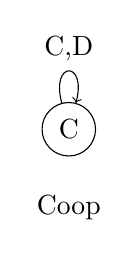
\begin{tikzpicture}
\node[draw, circle] (C) {C};
%\node[draw, circle] (D) [right of=C] {D};
\draw[->,loop above] (C) to node{C,D} (C);
%\draw[->] (C) to [bend left] (D);
%\draw[->] (D) to [bend left] (D);
\node[below of=C] {Coop};
\end{tikzpicture}
\hspace{2cm}
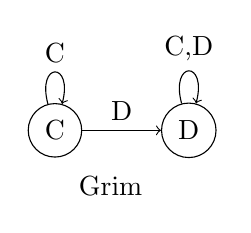
\begin{tikzpicture}
\node[draw, circle] (C) {C};
\node[draw, circle] (D) [right = 1cm of C] {D};
\draw[->,loop above] (C) to node{C} (C);
\draw[->] (C) to node[above]{D} (D);
\draw[->,loop above] (D) to node{C,D} (D);
\node[below right of=C] {Grim};
\end{tikzpicture}
\]

Suppose Agent 1 knows Agent 2 has either Coop or Grim model.

%8th fig.
\bigskip
\section*{Chapter 7. Neural Network}

\[ f_k(x_{k-1};\theta^k) = g_k(W_k^T x_{k-1} + b_k), \quad W_k \in \mathbb{R}^{d_{k-1} \times d_k}, \, x_{k-1} \in \mathbb{R}^{d_{k-1}}, \, b_k \in \mathbb{R}^{d_k} \]

Goal: \( \theta^* \in \arg\min L(\theta) \), Compute parameters \( \theta^* \) to minimize \( L(\theta) \)

\[ \text{MSE}: \, L(\theta) = \frac{1}{B} \sum_{k=1}^B \left( V^\pi(s_k) - V^\wedge(s_k;\theta) \right)^2 \]

Vanilla gradient descent is too costly,

SGD: \( \theta \leftarrow \theta - \alpha \nabla_\theta L(\theta|d) \big|_{d \sim \mathcal{D}} \), \( d \) drawn from dataset \( \mathcal{D} \).

Mini-batch: \( \theta \leftarrow \theta - \alpha \nabla_\theta L(\theta|B), \, B = \{d_i \sim \mathcal{D}\}_{i=1}^B \)

trade-off between converge fast and less variance.

\bigskip

\section*{Chapter 8. Deep Reinforcement Learning}

\[ Q(s^t,a^t) \leftarrow Q(s^t,a^t) + \alpha \left( r^t + \gamma \max_{a'} Q(s^{t+1},a') - Q(s^t,a^t) \right) \]

Define a neural network that receives state \( s \) as input, and outputs its estimated action value for each possible action.

\[ s \to \begin{bmatrix} Q(s,a_1;\theta) \\ \vdots \\ Q(s,a_{|A|};\theta) \end{bmatrix} \]

Loss function \( L(\theta) = \left( y^t - Q(s^t,a^t;\theta) \right)^2 \)

To ensure state values for terminal states are always 0,

we can set \( y^t = \begin{cases} r^t & \text{if } s^{t+1} \text{ is terminal} \\ r^t + \gamma \max_{a'} Q(s^{t+1},a';\theta) & \text{otherwise} \end{cases} \)

\[ Q(s^{t+1},a';\theta) = 0 \quad \andy{\text{Why setting } y^t = r^t \text{ can ensure this.}} \]

%9th fig.
\bigskip
\section*{Algorithm 10}
\begin{enumerate}
    \item Initialize value network \( Q \) with random parameters \( \theta \)
    \item Same for all algorithms
    \item Choose \( a^t \in \arg\max_a Q(s^t, a; \theta) \)
    \item Apply action \( a^t \); observe reward \( r^t \) and next state \( s^{t + 1} \)
    \item If \( s^{t + 1} \) is terminal then
    \item Target \( y^t \leftarrow r^t \) \andy{computed by bootstrapping}
    \item Else Target \( y^t \leftarrow r^t + \gamma \max_{a'} Q(s^{t + 1}, a'; \theta) \) \andy{$\leftarrow$ moving target problem}
    \item Loss \( L(\theta) \leftarrow (y^t - Q(s^t, a^t; \theta))^2 \)
    \item Update parameters \( \theta \)
\end{enumerate}

\noindent
A solution to this problem is by using another network, target network which periodically updates the parameters. Not too far from the estimates, and stays unchanged for a while.

\bigskip

\noindent
\textbf{Algorithm 11 Deep Q-Learning with target network}
\begin{enumerate}
    \item Initialize main network \( Q \) with random parameters \( \theta \)
    \item Initialize target network \( \bar{\theta} = \theta \)
    \item \textit{Same as algorithm 10}
    \item Else: Target \( y^t \leftarrow r^t + \gamma \max_{a'} Q(s^{t + 1}, a'; \bar{\theta}) \)
    \item Loss \( L(\theta) \leftarrow (y^t - Q(s^t, a^t; \theta))^2 \)
    \item Update \( \theta \)
    \item In a given interval, update \( \bar{\theta} \)
\end{enumerate}

\noindent
A phenomenon in Deep Learning is called catastrophic-forgetting, which is that updating the value function with the experience samples from the most recent episodes might cause the agent to forget how it arrived here (former experience). \\
To handle this problem, we might use a replay buffer \( D \) which stores experiences and train the model by randomly sample experiences from \( D \).

%10th fig.
\bigskip
\section*{Algorithm 12. Deep-Q-Network}
\begin{enumerate}
    \item Initialize \( Q \) with \( \theta \)
    \item Target network \( \bar{\theta} = \theta \)
    \item Empty replay buffer \( D = \{ \} \)
    \item \textit{Same for all}
    \item Otherwise: choose \( a^t \in \arg\max_a Q(s^t, a; \theta) \)
    \item Apply \( a^t \) and observe \( r^t, s^{t + 1} \)
    \item Store transition \( (s^t, a^t, r^t, s^{t + 1}) \) to \( D \)
    \item Sample random mini-batch \( B \) from \( D \). \( B = (s^k, a^k, r^k, s^{k + 1}) \)
    \item If \( s^{k + 1} \) is terminal:
    \item \( y^k \leftarrow r^k \)
    \item else:
    \item \( y^k \leftarrow r^k + \gamma \max_{a'} Q(s^{k + 1}, a'; \bar{\theta}) \)
    \item Loss \( L(\theta) \leftarrow \frac{1}{D} \sum_{k = 1}^D (y^k - Q(s^k, a^k; \theta))^2 \)
    \item Update parameters \( \theta \)
    \item In a interval, update \( \bar{\theta} \)
\end{enumerate}

\bigskip

\noindent
\section*{8.2 Why use policy gradient algorithms?}
\begin{enumerate}
    \item Able to represent probabilistic equilibrium
    \item Able to handle continuous action space.
\end{enumerate}

\noindent
To represent a probabilistic policy for discrete action spaces using neural networks, the network receives a state as input and outputs a scalar \( (s, a) \) for all \( a \in A \) then put them in a softmax function:
\[
\pi(a|s; \phi) = \frac{e^{U(s, a)}}{\sum_{a' \in A} e^{U(s, a')}}
\]

\noindent
\textbf{Policy Gradient Theorem}:
\[
\nabla_\phi J(\phi) \propto \sum_{s \in S} P_r(s|\pi) \sum_{a \in A} Q^\pi(s, a) \nabla_\phi \pi(a|s; \phi)
\]

\noindent
\( J \) represents the quality of a policy \( \pi \) with parameters \( \phi \), therefore, we want to maximize it.

\[
= \mathbb{E}_{s \sim P_r(s|\pi), a \sim \pi(\cdot|s; \phi)} \left[ Q^\pi(s, a) \nabla_\phi \log \pi(a|s; \phi) \right]
\]

\noindent
This expectation also clearly illustrates the restriction that optimization of parametrized policy is limited to on-policy data, that is, the data used to optimize \( \pi \) is generated by policy \( \pi \) itself.

\noindent
We need to either approximate the derived expectation or obtain samples from it.

%11th fig.
\bigskip
\section*{Algorithm REINFORCE}
\begin{enumerate}
    \item Initialize policy network \( \pi \) with random parameters \( \phi \)
    \item Repeat for every episode:
    \item For time \( t = 0 \cdots T - 1 \) do:
    \item Observe \( s_t \)
    \item Sample action \( a_t \sim \pi(\cdot|s_t; \phi) \)
    \item Apply \( a_t \) and observe \( r_t \) and \( s_{t + 1} \)
    \item Loss \( \mathcal{L}(\phi) \leftarrow -\frac{1}{T} \sum_{t = 0}^{T - 1} \left( \sum_{\tau = t}^{T - 1} \gamma^{\tau - t} r_\tau \right) \log \pi(a_t|s_t; \phi) \)
    \item Update \( \phi \) by minimizing \( \mathcal{L}(\phi) \)
\end{enumerate}

\bigskip

\noindent
\section*{8.2.3 REINFORCE: Monte Carlo Policy Gradient \andy{ baseline???}}

\bigskip

\noindent
\textbf{Actor-Critic Algorithm} \\
Actor-Critic is a family of algorithms that trains a parametrized policy called actor, and a value function called critic, alongside each other, able to update the policy in a single time step rather than episode. \\
Trade-off is that has higher variance. \\
Single step \( \longleftarrow \) N-step \( \longleftarrow \) Entire episode \\
Actor-Critic \quad \quad \quad \quad \quad \quad MC

\bigskip

\noindent
\textbf{Advantage Actor-Critic} \\
\( \text{Adv}^\pi(s, a) = Q^\pi(s, a) - V^\pi(s) \) \\
\( Q^\pi(s, a) \): At state \( s \), do action \( a \), then follow \( \pi \) \\
\( V^\pi(s) \): At state \( s \), directly follow \( \pi \).

\[
Q(s^t, a^t) = \begin{cases} 
r^t & \text{if } s^{t + 1} \text{ is terminal} \\
r^t + \gamma V(s^{t + 1}) & \text{otherwise}
\end{cases}
\]

\bigskip

\noindent
\textbf{Algorithm 14 Simplified advantage actor critic}
\begin{enumerate}
    \item Initialize actor (policy) network \( \pi \) with para \( \phi \)
    \item Initialize critic (state-value) network \( V \) with para \( \theta \)
    \item Repeat for every episode
    \item For time step \( t = 0,1,2\cdots \) do
    \item Observe \( s_t \)
    \item Sample action \( a_t \sim \pi(\cdot|s_t; \phi) \)
    \item Apply \( a_t \), observe \( r_t \) and \( s_{t + 1} \)
    \item If \( s_{t + 1} \) is terminal then
    \item \( \text{Adv}(s_t, a_t) \leftarrow r_t - V(s_t; \theta) \)
    \item Critic target \( y_t \leftarrow r_t \)
    \item else
    \item \( \text{Adv}(s_t, a_t) \leftarrow r_t + \gamma V(s_{t + 1}; \theta) - V(s_t; \theta) \)
    \item Critic target \( y_t \leftarrow r_t + \gamma V(s_{t + 1}; \theta) \)
    \item actor loss \( \mathcal{L}(\phi) \leftarrow -\text{Adv}(s_t, a_t) \log \pi(a_t|s_t; \phi) \)
    \item critic loss \( \mathcal{L}(\theta) \leftarrow (y_t - V(s_t; \theta))^2 \)
    \item Update \( \phi \)
    \item Update \( \theta \)
\end{enumerate}

%12th fig.
\bigskip
\section*{9.1.3 Centralized Training with Decentralized Execution (CTDE)}
\begin{itemize}
    \item Centralized training and decentralized execution (CTDE): used (centralized training to train agent policies, while each agent's policy itself only requires the agent's local observation.
\end{itemize}

\bigskip

\noindent
\textbf{Algorithm 17 Independent deep Q-networks. (Similar to DQN)}
\begin{enumerate}
    \item Initialize \( n \) value networks with random \( \theta_1, \cdots, \theta_n; \theta \)
    \item Initialize \( n \) target networks with \( \bar{\theta}_1 = \theta_1, \cdots, \bar{\theta}_n = \theta_n \)
    \item Initialize \( n \) replay buffers \( D_1, \cdots, D_n \)
    \item For time step \( t = 0, 1, 2, \cdots \) do
    \item Collect observations \( o_1^t, \cdots, o_n^t \)
    \item For agent \( i = 1, \cdots, n \) do
    \item \( \varepsilon \)-greedy explore
    \item Otherwise: choose \( a_i^t \in \arg\max_{a_i} Q_i(o_i^t, a_i; \theta_i) \)
    \item Apply actions \( (a_1^t, \cdots, a_n^t) \); collect rewards \( r_1^t, \cdots, r_n^t \) and next observations \( o_1^{t + 1}, \cdots, o_n^{t + 1} \)
    \item For agent \( i = 1, \cdots, n \) do
    \item Store \( (o_i^t, a_i^t, r_i^t, o_i^{t + 1}) \) to \( D_i \)
    \item Sample random mini-batch of \( B \)-transitions \( (o_i^k, a_i^k, r_i^k, o_i^{k + 1}) \) from \( D_i \)
    \item If \( o_i^{k + 1} \) is terminal then
    \item Target \( y_i^k \leftarrow r_i^k \)
    \item else
    \item \( y_i^k \leftarrow r_i^k + \gamma \max_{a_i'} Q_i(o_i^{k + 1}, a_i'; \bar{\theta}_i) \)
    \item Loss \( \mathcal{L}(\theta_i) \leftarrow \frac{1}{B} \sum_{k = 1}^B \left( y_i^k - Q_i(o_i^k, a_i^k; \theta_i) \right)^2 \)
    \item Update \( \theta_i \) by minimizing \( \mathcal{L}(\theta_i) \)
    \item In a interval, update \( \bar{\theta}_i \)
\end{enumerate}

\bigskip

\noindent
\textbf{Multi-agent policy gradient theorem}
\[
\nabla_{\phi_i} J(\phi_i) \propto \mathbb{E}_{h \sim P_h(\cdot|\pi), a_i \sim \pi_i, a_{-i} \sim \pi_{-i}} \left[ Q_i^\pi(h, \langle a_i, a_{-i} \rangle) \nabla_{\phi_i} \log \pi_i(a_i|h_i = o_i^t(h); \phi_i) \right]
\]

\bigskip

\noindent
\textbf{Once the training is completed}, the Critic network is no longer utilized. Therefore, there's no requirement for a decentralized critic network. So we can define critic as \( V(h_1^t, \cdots, h_n^t; \theta_i) \) for agent \( i \), value loss of estimated critic, becomes \( \mathcal{L}(\theta_i) = (y_i - V(h_i^t, z^t; \theta_i))^2 \) with \( y_i = r_i^t + \gamma V(h_i^{t + 1}, z^{t + 1}; \theta_i) \)

\bigskip

\noindent
\section*{9.4.3 Centralized Action-Value Critics} 
For each agent \( i \), trains a policy \( \pi_i \) which is Conditioned on agent \( i \)'s observation history, For the critic, agent \( i \) trains an action-value function \( Q \) that is conditioned on individual observation history, Centralized information, and actions of all agents.

\[
\mathcal{L}(\theta_i) = \left( y_i - Q(h_i^t, z^t, a^t; \theta_i) \right)^2 \text{ with } y_i = r_i^t + \gamma Q(h_i^{t + 1}, z^{t + 1}, a^{t + 1}; \theta_i)
\]

\[
\text{policy loss } \mathcal{L}(\phi_i) = -Q(h_i^t, z^t, a^t; \theta_i) \log \pi_i(a^t|h_i^t; \phi_i)
\]

\( \mathcal{L}(\theta_i) \) is value loss, \( \mathcal{L}(\phi_i) \) is policy loss.

\bigskip

\noindent
\textbf{Why training action-value critic \( Q(h_i, z, a; \theta_i) \) instead of centralized value function \( V(h_i, z; \theta_i) \)?} To directly estimate the impact of the action selection on expected return. \( z \) is Centralized information. \\
Possibly more difficult to train, more outputs.

%13th fig.
\bigskip
\textbf{No conflict game}: \( \arg\max_i U_i(\pi) = \arg\max_j U_j(\pi) \quad \forall i, j \in \mathcal{I} \)

\bigskip

\noindent
\section*{9.5 Value Decomposition in Common-Reward Games} 

Value decomposition algorithms decompose optimized action-value function into simpler functions that can be learned more efficiently and enable decentralized execution. Called, “utility function”, “jointly optimized”.

\noindent
\textbf{IGM (Individual-global-max) property}: States that the greedy joint actions with respect to (centralized action-value function) equal to individual actions of all agents that maximize the respective individual utilities.

\noindent
Define: 
\[
A^* (h, z; \theta) = \arg\max_{a \in A} Q(h, z, a; \theta)
\]
\[
A_i^* (h_i, z; \theta_i) = \arg\max_{a_i \in A_i} Q_i(h_i, z, a_i; \theta_i)
\]

\noindent
IGM: \( \forall a = (a_1 \cdots a_n) \in A, a \in A^*(h, z; \theta) \iff \forall i \in \mathcal{I}, a_i \in A_i^*(h_i; z; \theta_i) \)

\noindent
Can address multi-agent credit assignment problem.

\noindent
Simple approach: \( Q(h^t, z^t, a^t; \theta) = \sum_{i \in \mathcal{I}} Q_i(h^t, a^t; \theta_i) \)

\bigskip

\noindent
\textbf{Algorithm 21 Value decomposition networks (VDN)}
\begin{enumerate}
    \item Initialize \( n \) utility networks \( \theta_1 \cdots \theta_n \)
    \item Initialize \( n \) target networks \( \bar{\theta}_1 = \theta_1 \cdots \bar{\theta}_n = \theta_n \)
    \item Initialize a shared replay buffer \( D \)
    \item For time step \( t = 0,1,2\cdots \) do
    \item Collect observations \( o_1 \cdots o_n \)
    \item For agent \( i = 1\cdots n \) do
    \item With probability \( \varepsilon \): choose random \( a_i^t \)
    \item Otherwise: choose \( a_i^t \in \arg\max_{a_i} Q_i(h_i^t, a_i; \theta_i) \)
    \item Apply actions, collect timed reward \( r^t \) and next observations \( o_1^{t + 1} \cdots o_n^{t + 1} \)
    \item Store \( (h^t, a^t, r^t, h^{t + 1}) \) in \( D \)
    \item Sample \( B = (h^k, a^k, r^k, h^{k + 1}) \) from \( D \)
    \item If \( s^{k + 1} \) is terminal then
    \item \( y^k \leftarrow r^k \)
    \item else
    \item \( y^k \leftarrow r^k + \gamma \sum_{i \in \mathcal{I}} \max_{a_i'} Q_i(h_i^{k + 1}, a_i'; \bar{\theta}_i) \)
    \item Loss \( \mathcal{L}(\theta) \leftarrow \frac{1}{B} \sum_{k = 1}^B \left( y^k - \sum_{i \in \mathcal{I}} Q_i(h^k, a^k; \theta_i) \right)^2 \)
    \item Update \( \theta \) by minimizing \( \mathcal{L}(\theta) \)
    \item In a set interval, update \( \bar{\theta}_i \) for each \( i \)
\end{enumerate}

\bigskip

\noindent
Need not to be linear in practice, IGM satisfies as long as
\[
\forall i \in \mathcal{I}, \forall a \in A: \frac{\partial Q(h, z, a; \theta)}{\partial Q(h, z, a_i; \theta_i)} > 0 \quad Q \text{-MAX}
\]
For instance \( Q(h, z, a; \theta) = \sum_{i \in \mathcal{I}} Q_i(h, z, a_i; \theta_i) \) (for \( a = (a_1 \cdots a_n) \))

\bigskip
\noindent
Sufficient condition for IGM if
\[
\left( \sum_{i \in \mathcal{I}} Q_i(h, a_i; \theta_i) - \sum_{i \in \mathcal{I}} Q_i(h, a_i^{*'}; \theta_i) \right) + \left( \max_{a''} Q(h, z, a''; \theta) - Q(h, z, a; \theta) \right)
\]
\[
= \begin{cases} 
= 0 & \text{if } a = a^* \\
\geq 0 & \text{else}
\end{cases}
\]
where \( a_i^* = \arg\max_{a_i \in A_i} Q_i(h, z, a_i; \theta_i) \)

%14th fig.
\bigskip
\section*{9.6 Agent Modeling with Neural Networks} 

Agent \( i \) model agent \( j \), \( \hat{\pi}_j^i \) by minimizing the cross-entropy loss between the predicted value \( \hat{\pi}_j^i \) and true action \( j \)
\[
\mathcal{L}(\phi_j^i) = -\log \hat{\pi}_j^i(a_j^t|h_j^t; \phi_j^i)
\]

\noindent
Each agent also trains a centralized action-value function \( Q \) parametrized by \( \theta_i \) \\
Takes in \( h_i^t \) and \( a_{-i} \) as input, and outputs the estimated centralized action value for each action of \( i \). Loss of this function training:
\[
\mathcal{L}(\theta_i) = \frac{1}{B} \sum_{(h_i^t, a^t, r_i^t, h_i^{t + 1}) \in B} \left( r_i^t + \gamma \max_{a_i' \in A_i} AV(h_i^{t + 1}, a_i'; \bar{\theta}_i) - Q(h_i^t, a^t, a_i^t; \theta_i) \right)^2
\]

\noindent
\( AV = \text{Action Value} \)
\[
AV(h_i, a_i; \theta_i) = \sum_{a_{-i} \in A_{-i}} Q(h_i, \langle a_i, a_{-i} \rangle; \theta_i) \hat{\pi}_{-i}^i(a_{-i}|h_i; \phi_{-i}^i)
\]
\[
= \sum_{j \neq i} Q(h_i, \langle a_i, a_{-i} \rangle; \theta_i) \prod_{j \neq i} \hat{\pi}_j^i(a_j|h_j; \phi_j^i)
\]
\( \to \text{Actual Value} \)

\noindent
We can also estimate \( AV(h_i, a_i; \theta_i) \) by
\[
= \frac{1}{K} \sum_{k = 1}^K Q(h_i, \langle a_i, a_{-i}^k \rangle; \theta_i)
\]

\bigskip

\noindent
\section* {9.8 Policy Self-Play in Zero-Sum Games}

\noindent
\textbf{Algorithm 25 MCTS for MDPs}
\begin{enumerate}
    \item Repeat for every episode:
    \item For \( t = 1, 2, 3 \cdots \) do
    \item Observe current state \( s^t \)
    \item For \( k \) simulations do
    \item \( \tau \leftarrow t \)
    \item \( s^\tau \leftarrow s^t \) \quad \textit{//perform simulation}
    \item while \( s^\tau \) is non-terminal and \( s^\tau \)-node exists in tree do
    \item \( a^\tau \leftarrow \text{Explore Actions}(s^\tau) \)
    \item \( s^{\tau + 1} \sim T(\cdot|s^\tau, a^\tau) \)
    \item \( r^\tau \leftarrow R(s^\tau, a^\tau, s^{\tau + 1}) \)
    \item \( \tau \leftarrow \tau + 1 \)
    \item if \( s^\tau \)-node does not exist in tree then:
    \item Initialize Node \( (s^\tau) \): set counter \( N(s^\tau, a) = 0 \) and \( Q(s^\tau, a) = 0 \) for all \( a \in A \)
    \item while \( \tau > t \) do
    \item \( \tau \leftarrow \tau - 1 \)
    \item Update \( (s^\tau, a^\tau) \)
    \item Select action for \( s^t \)
    \item \( \pi^t \leftarrow \text{best Action}(s^t) \)
    \item \( a^t \sim \pi^t \)
\end{enumerate}

\end{document}
